\documentclass{article}
\usepackage[utf8]{inputenc}
\usepackage{graphicx, graphics, float}
\usepackage[a4paper, total={6in, 9in}]{geometry}
\usepackage[spanish]{babel}
\usepackage{subcaption}
\title{Haz Una Línea\\
\large Memoria DS - Práctica 3}
\author{Andrés Merlo Trujillo\\ Sergio Hervás Cobo\\ Javier Serrano Lucas\\ Ricardo Molina Rodríguez}

\begin{document}
\date{Abril 2022}
\maketitle
\section{Introducción}
En esta práctica se ha realizado una serie de pruebas para comprobar el funcionamiento correcto de
ciertas funcionalidades y métodos de la aplicación realizada en la Práctica 2 (Haz Una Línea). Se han implementado
tests de unidad que comprobarán si la ejecución de un método de una clase produce el resultado
esperado y tests de widgets que buscarán la existencia de algún elemento que permita verificar su buen funcionamiento.

En total se han realido 4 tests de widgets y 8 de unidad que explicaremos a continuación en los siguientes apartados.


\section{Tests de unidad}
\begin{itemize}
\item \textbf{El volumen de la música debería cambiar a 0:} Clase: Música.

Para este test se ha comprobado que el volumen de la música es 0 cuando se llama a "setSonido".
De esta forma se comprobará si de verdad el volumen del sonido cambia dentro de dicho método cuando el usuario aprieta el botón del cambio de volumen.

\item \textbf{El volumen de la música debería cambiar a 1:} Clase: Música.

Para este test se ha comprobado que el volumen de la música es 1 cuando se llama a "setSonido" dos veces.
De esta forma se comprobará si de verdad el volumen del sonido cambia dentro de dicho método cuando el usuario aprieta dos veces el botón del cambio de volumen.

\item \textbf{La pieza no se debe mover en los bordes del tablero:} Clase: Pieza

Este test verifica si al mover una pieza que está en el borde del tablero en esa misma dirección, esta permanece en el mismo sitio sin salirse del tablero. Se hace
comprobando cada pieza que puede existir en el tablero y mirando si sus coordenadas están dentro de las del tablero.

\item \textbf{La bomba explota:}Clase: PiezaBomba.

Este test se encarga de comprobar que las piezas bombas al detonar eliminan los bloques colindantes a los propios bloques de la pieza bomba.
\item \textbf{La pieza esta en el suelo:} Clase: Pieza.

Este test comprueba que la pieza al bajarla se encuentre en el suelo del tablero y no se haya pasado más de la cuenta.
\item \textbf{Todas las piezas creadas son distintas:} Clase: Factoria

Este test comprueba que el algoritmo usado en la factoria para obtener las piezas es consistente. Se ha hecho un algoritmo tipo ``saco'', en el que un tipo de pieza no vuelve a salir hasta que no salgan las demás. Por tanto este test se encarga de comprobar que las 7 primeras piezas son distintas, como es de esperar.

\item \textbf{La pieza detecta colision con otra de abajo:} Clase: Pieza
Este test se encarga de comprobar que al poner una pieza encima de otra no la atraviese y detecte correctamente la colisión.
%COMPROBAR MAÑANA
\item \textbf{Cuando se forman 10 bloques horizontales se destruye una linea:} Clase: Tablero

Este test consiste en colocar 10 bloques (en este caso 5 cubos) y comprobar que al hacer la línea (2 en esta ocasión) se eliminan del tablero. Se ha realizado una modificación
en la clase Tablero para poder instanciarlo, ya que al ser un State, la clase es privada por defecto.
\end{itemize}


\section{Tests de Widgets}
\begin{itemize}
\item \textbf{Cambio de icono al apagar/encender la musica:} Clase: Música.

\item \textbf{Aparece la pantalla de Game Over:} Clase: GameOver.

\item \textbf{Al salir de la partida desde el menú de pausa regresa al menú principal:} Clase: Pausa

\item \textbf{Al reservar pieza, esta aparece en la pantalla:}Clase: Tablero.

\end{itemize}
\begin{figure}[H]
  \begin{subfigure}{0.5\textwidth}
          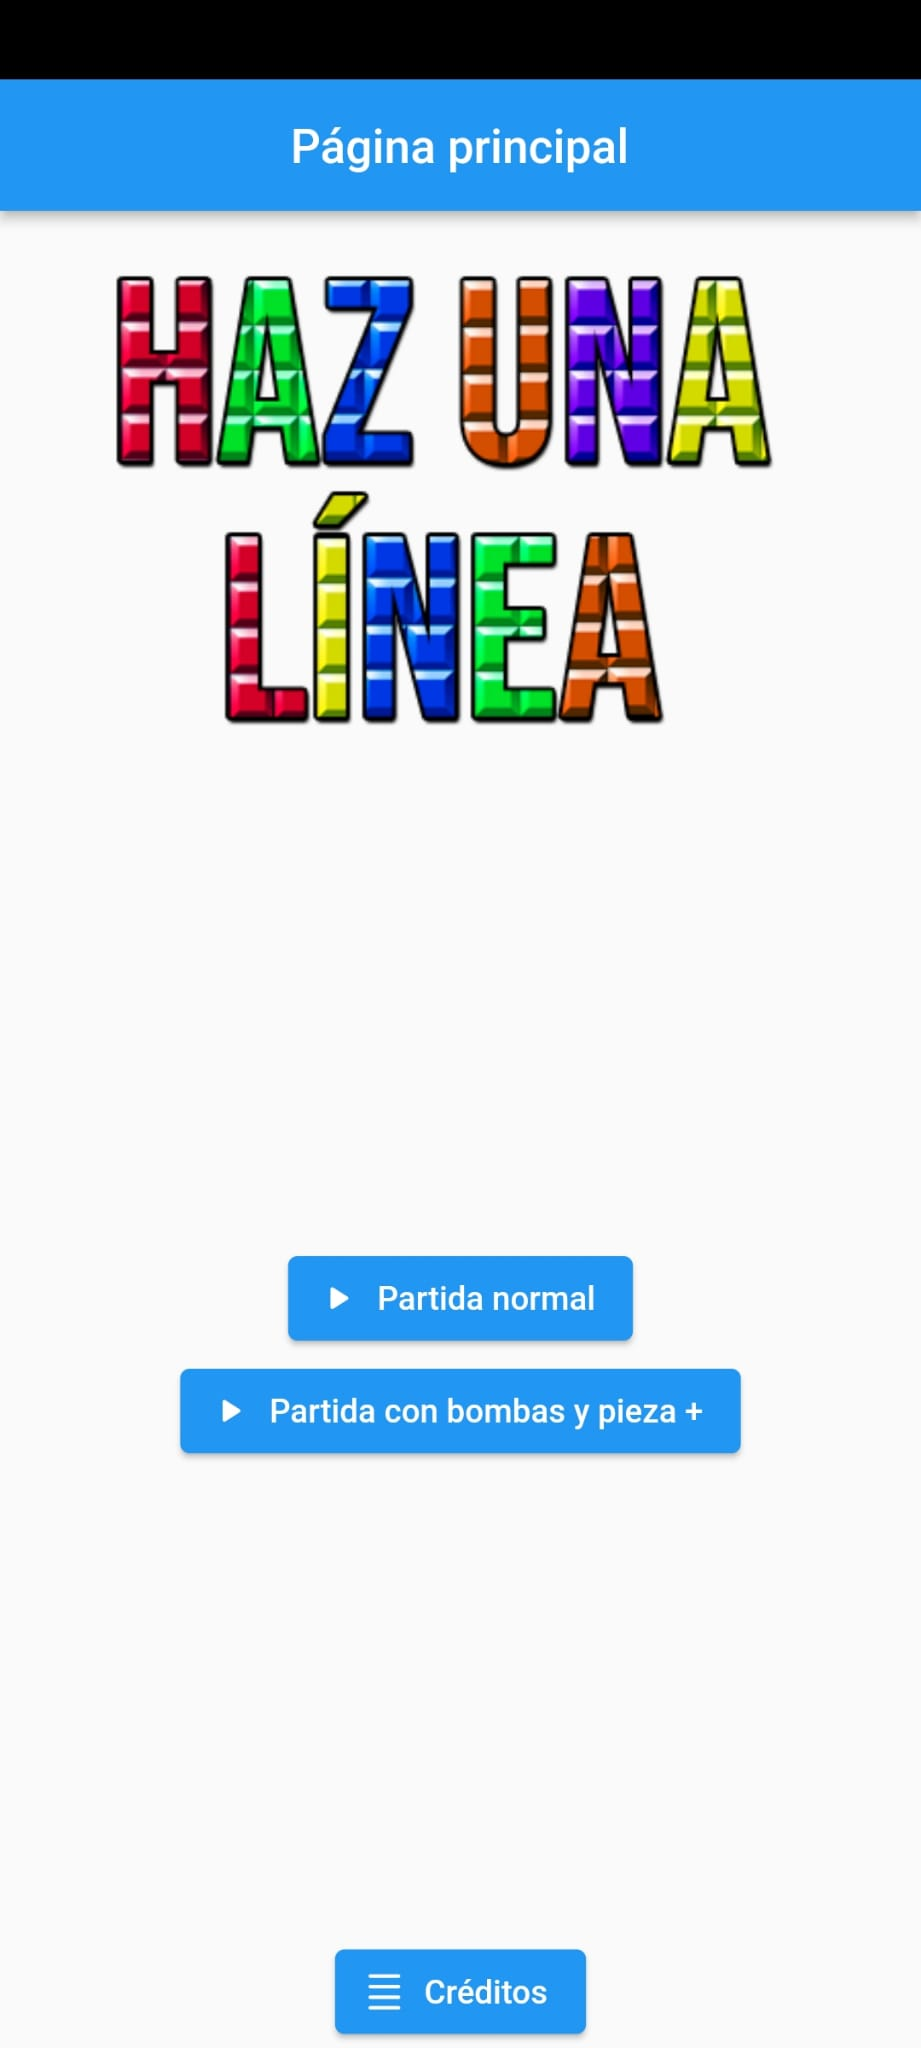
\includegraphics[width=\textwidth]{imagenes/captura7.jpeg}
          \caption{Modo claro}
  \end{subfigure}
  \begin{subfigure}{0.5\textwidth}
          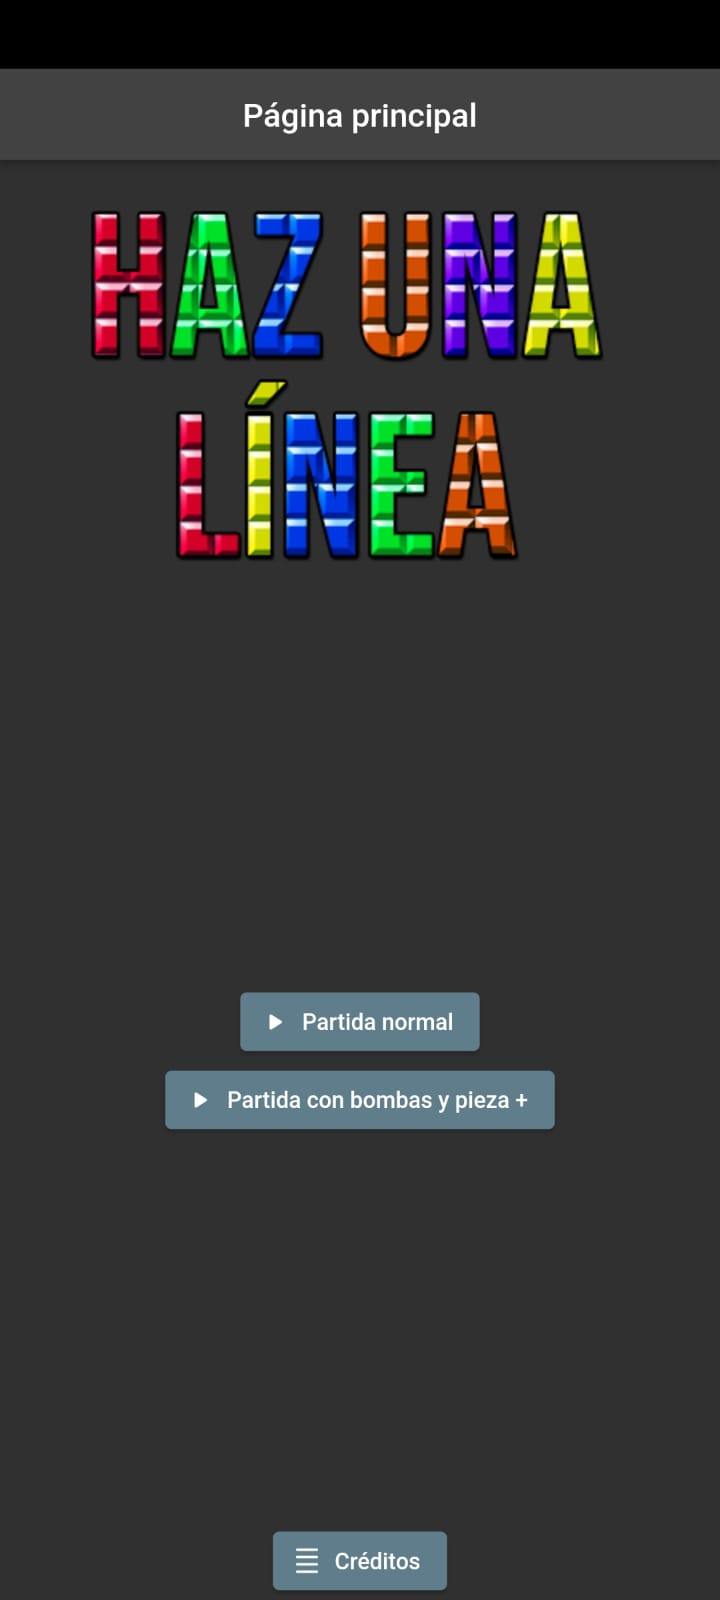
\includegraphics[width=\textwidth]{imagenes/captura1dark.jpeg}
          \caption{Modo oscuro}
  \end{subfigure}
  \caption{Pantalla de inicio de la aplicación.}
\end{figure}

\begin{figure}[H]
  \begin{subfigure}{0.5\textwidth}
          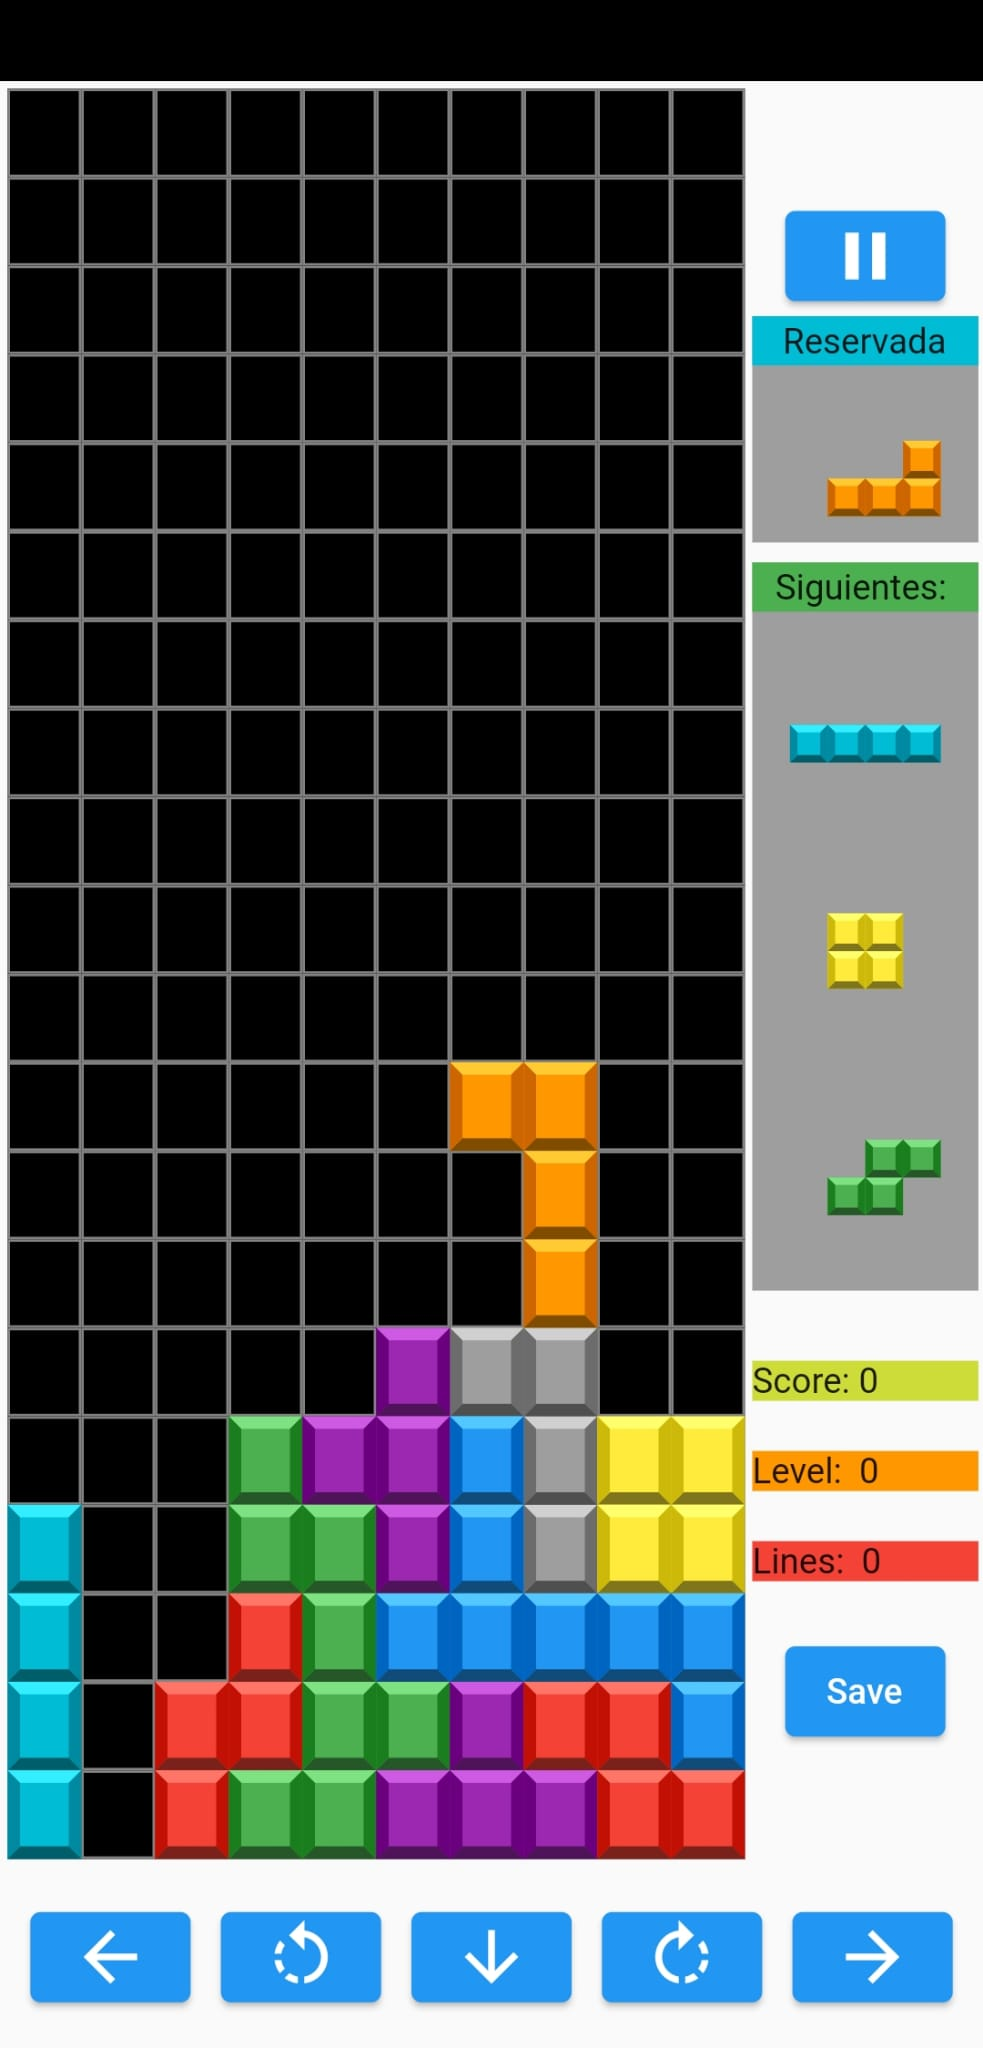
\includegraphics[width=\textwidth]{imagenes/captura1.jpeg}
          \caption{Modo claro}
  \end{subfigure}
  \begin{subfigure}{0.5\textwidth}
          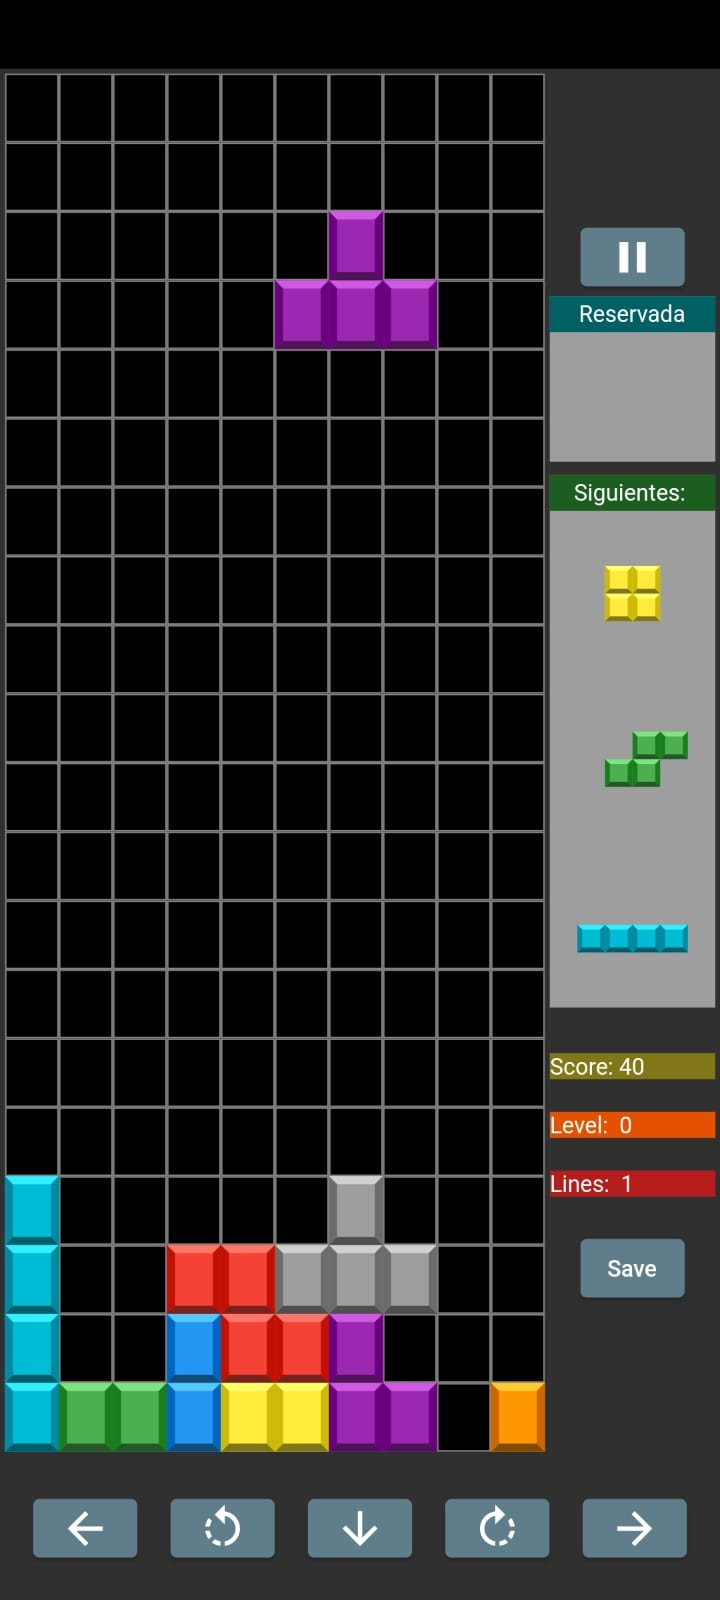
\includegraphics[width=\textwidth]{imagenes/captura2dark.jpeg}
          \caption{Modo oscuro}
  \end{subfigure}
  \caption{Ejemplo de tablero.}
\end{figure}

\begin{figure}[H]
  \begin{subfigure}{0.5\textwidth}
          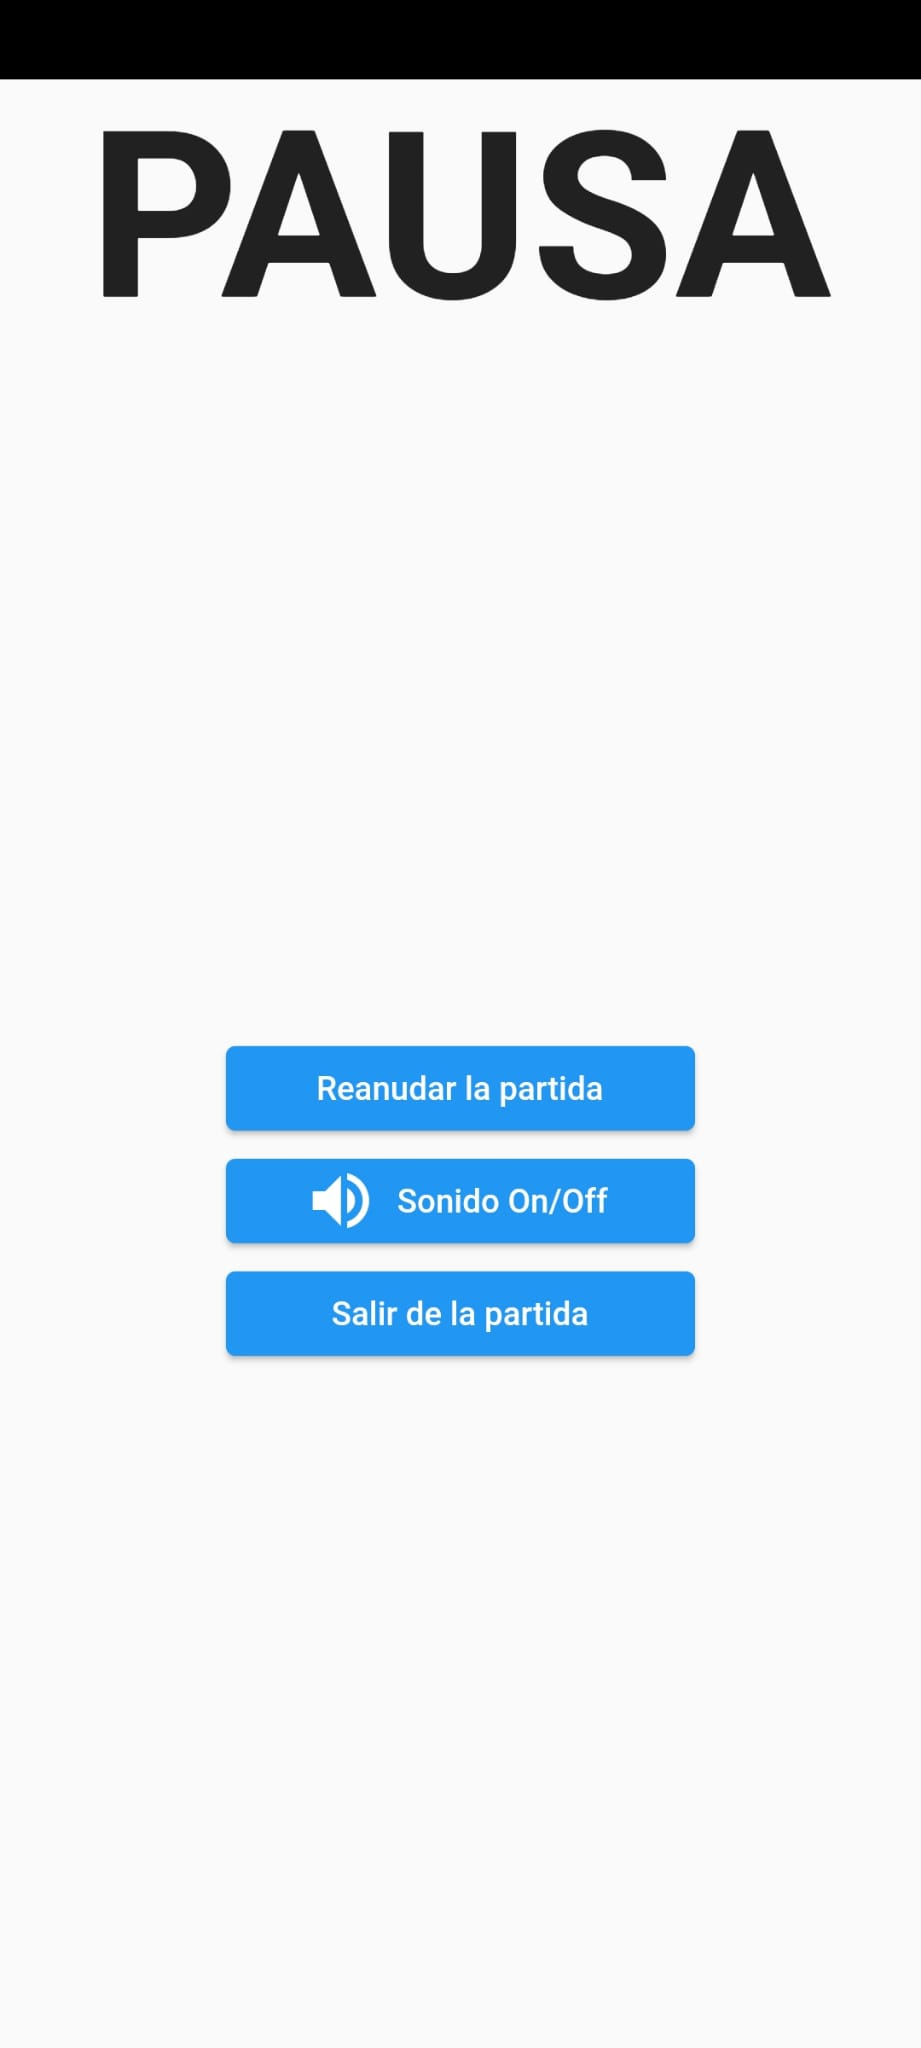
\includegraphics[width=\textwidth]{imagenes/captura6.jpeg}
          \caption{Modo claro}
  \end{subfigure}
  \begin{subfigure}{0.5\textwidth}
          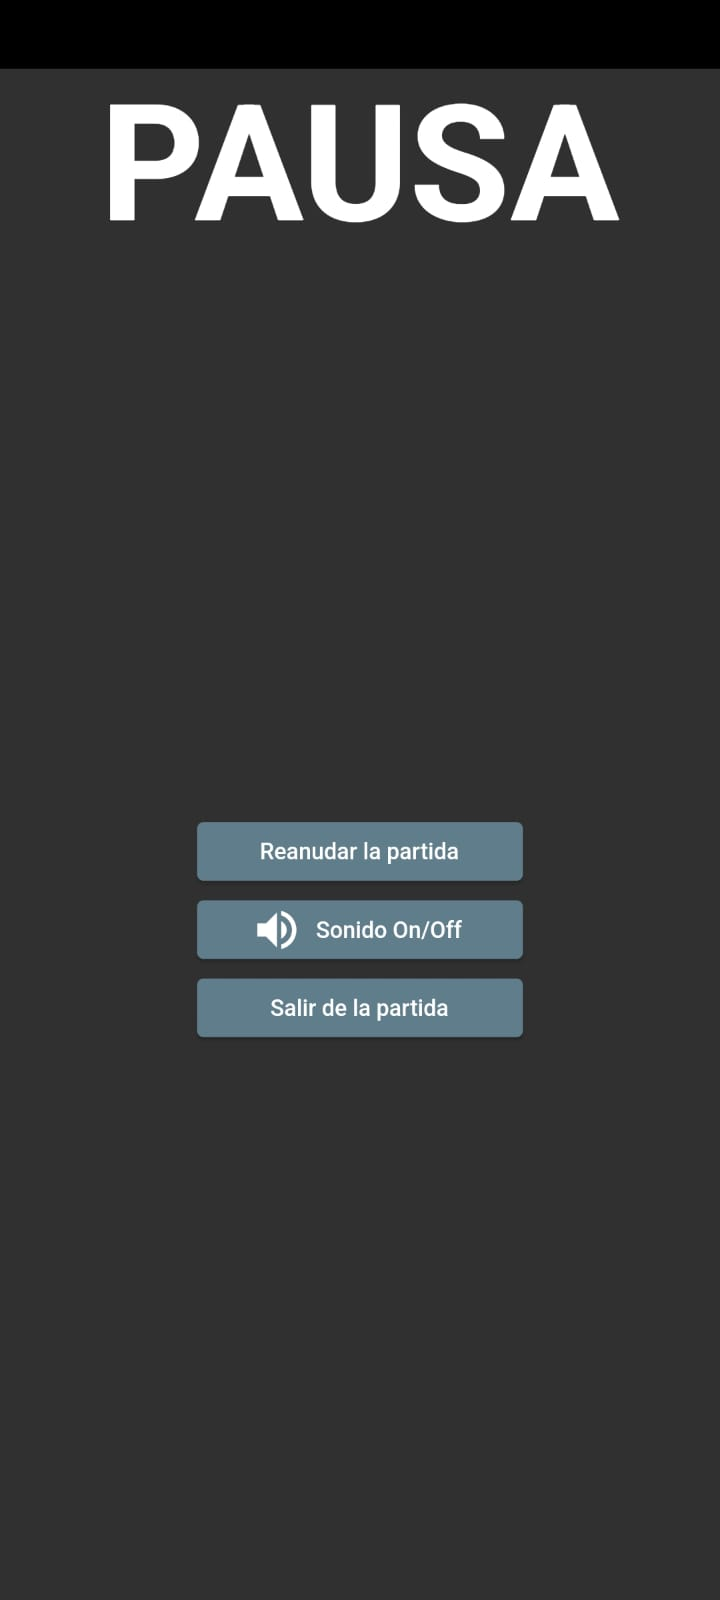
\includegraphics[width=\textwidth]{imagenes/captura3dark.jpeg}
          \caption{Modo oscuro}
  \end{subfigure}
  \caption{Pausa del juego.}
\end{figure}

\begin{figure}[H]
  \begin{subfigure}{0.5\textwidth}
          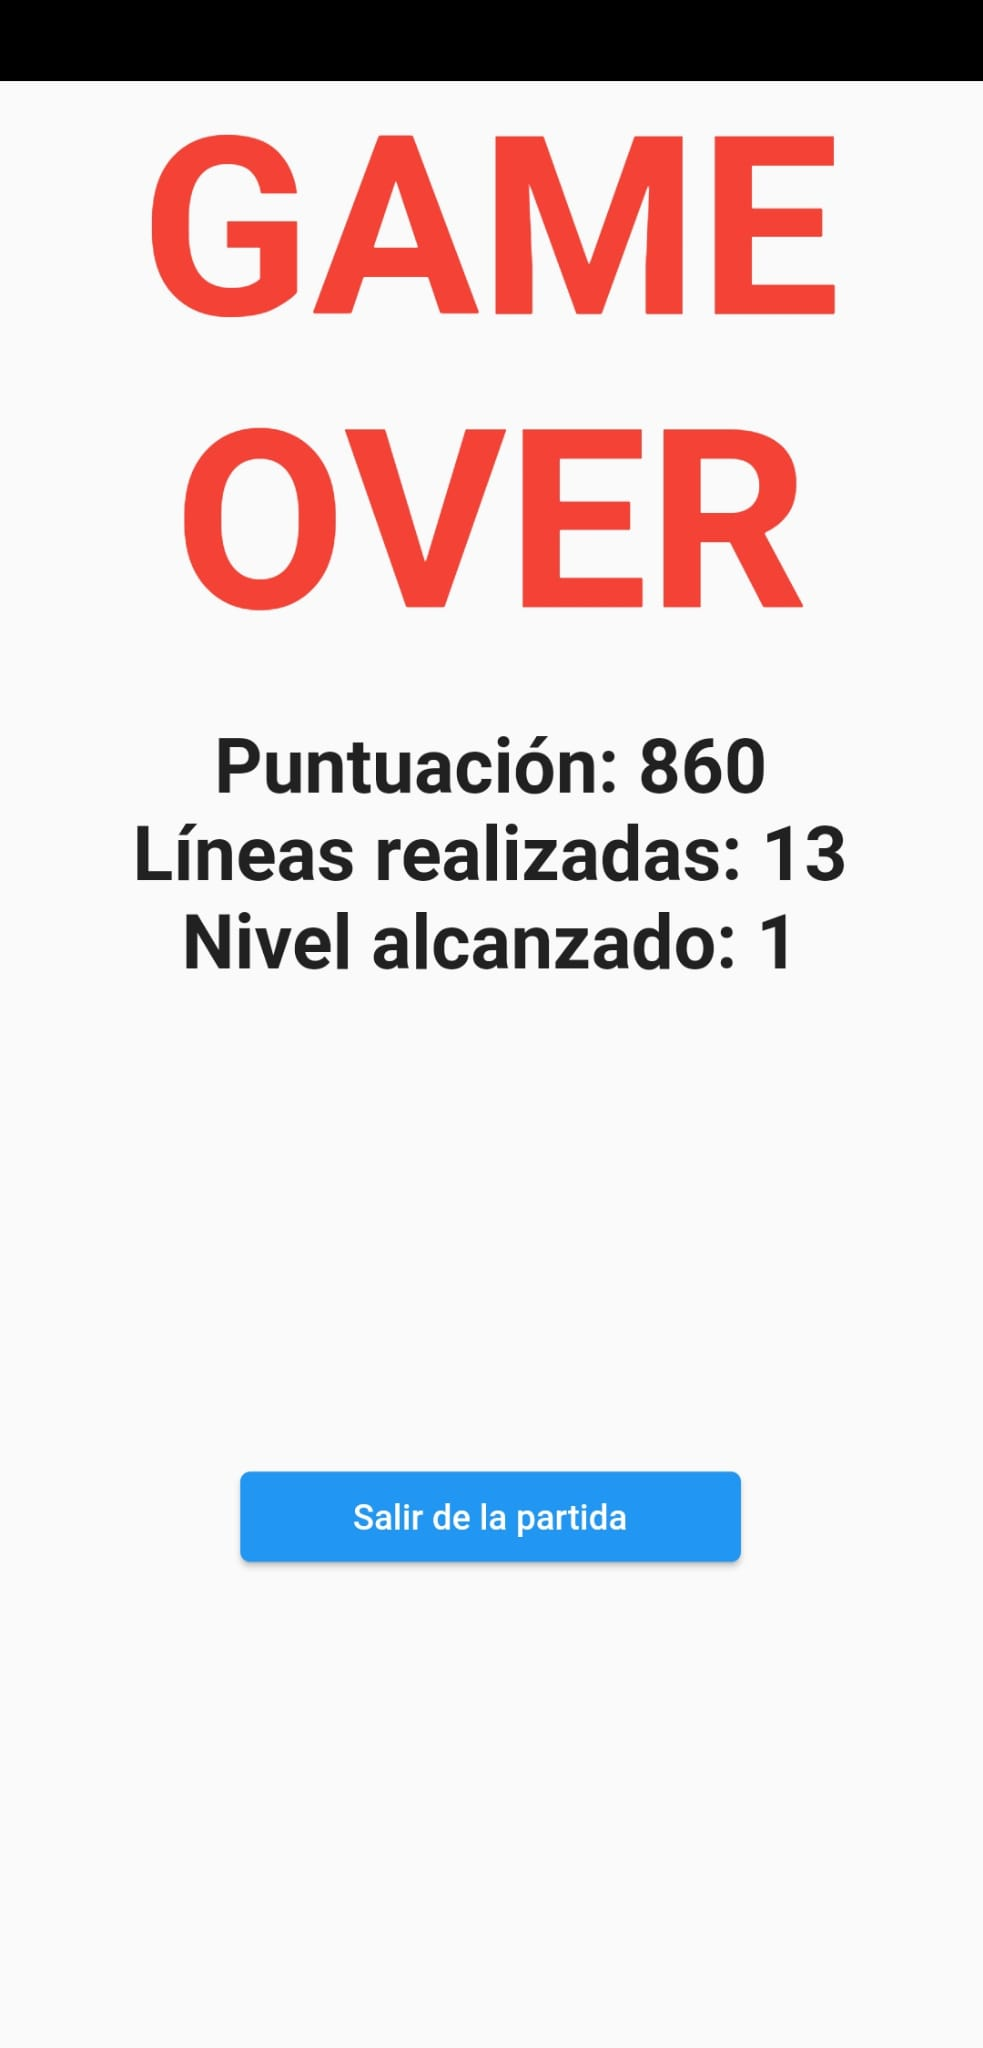
\includegraphics[width=\textwidth]{imagenes/captura4.jpeg}
          \caption{Modo claro}
  \end{subfigure}
  \begin{subfigure}{0.5\textwidth}
          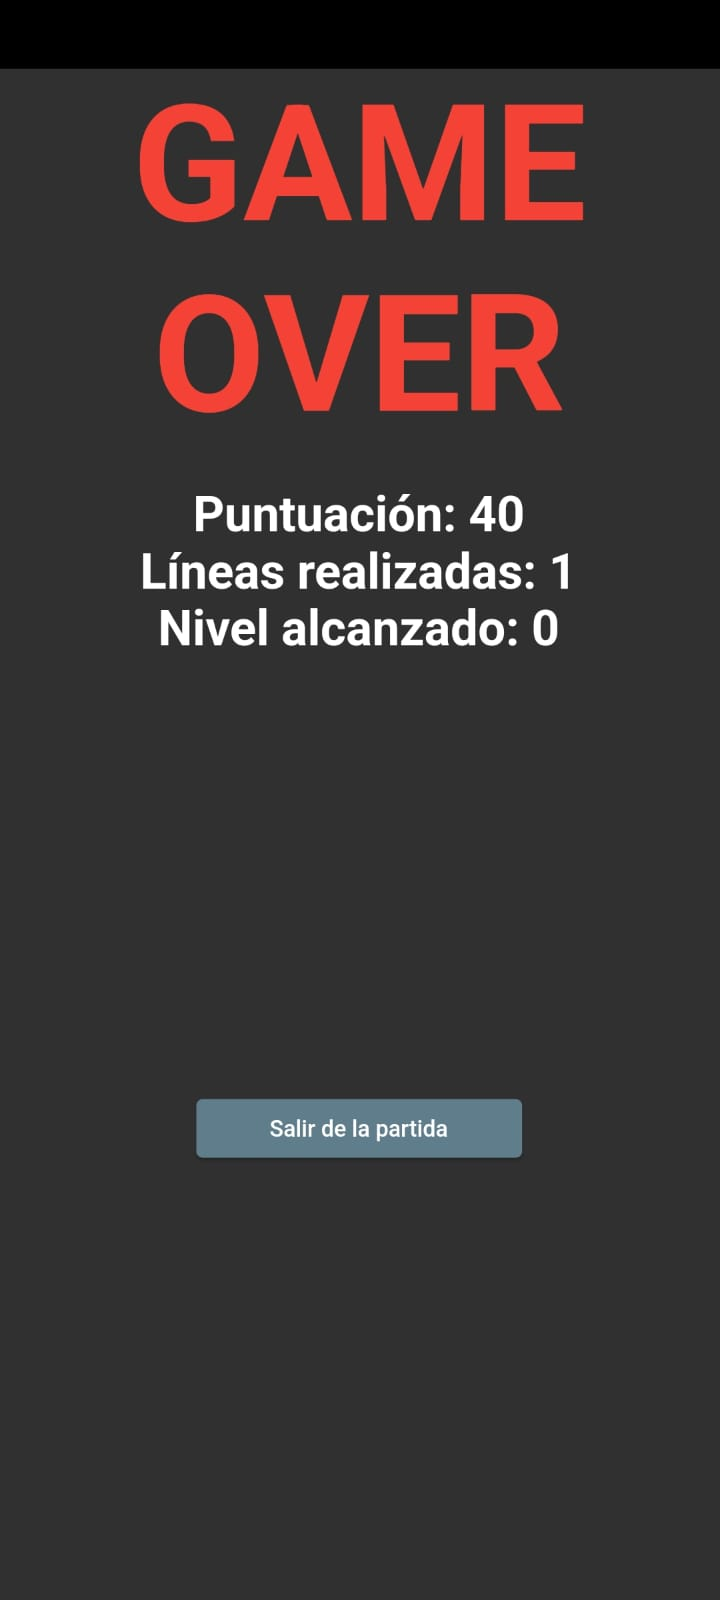
\includegraphics[width=\textwidth]{imagenes/captura4dark.jpeg}
          \caption{Modo oscuro}
  \end{subfigure}
  \caption{Pantalla de Game Over}
\end{figure}


\end{document}
